\documentclass{standalone}
\usepackage{tikz}
\usepackage{ctex,siunitx}
\usepackage{tkz-euclide}
\usepackage{amsmath}
\usetikzlibrary{patterns, calc}
\usetikzlibrary {decorations.pathmorphing, decorations.pathreplacing, decorations.shapes,}
\begin{document}
\small
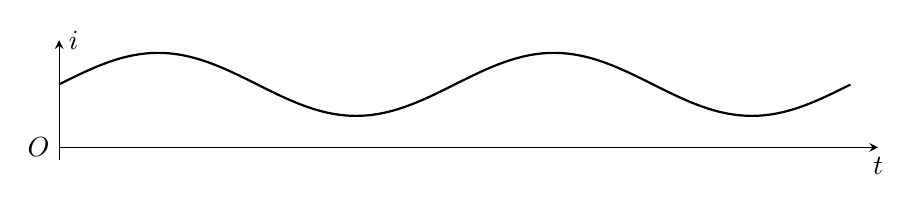
\begin{tikzpicture}[>=stealth, scale=0.8, domain=0:4*pi, samples=2000]
  \useasboundingbox(-0.5,1.9)rectangle(13.2,-0.5);
  \draw [->](0,0)node [left]{$O$}--(13,0) node [below]{$t$};
  \draw [->](0,-0.2)--(0,1.7) node [right]{$i$};
  % \draw [thick, domain=0:4*pi]  plot (\x,{(0.5*sin(\x r)+1)*cos(20*\x r)});
  \draw [thick, domain=0:4*pi]  plot (\x,{0.5*sin(\x r)+1});
  % \draw [densely dashed, domain=0:4*pi]  plot (\x,{-0.5*sin(\x r)-1});
\end{tikzpicture}
\end{document}